\chapter{Pflichtenheft}
\section{Einleitung/Aufgabenstellung}
Mit dem Projekt 'Battletanks' soll im Rahmen des Softwarepraktikums Informatik der Universität Würzburg im Wintersemester 2016/17 ein Desktop-basiertes Multiplayerspiel erstellt werden.
In diesem Spiel können bis zu vier Spieler mit je einer Spielfigur in einem Top Down 2D Spielfeld gegeneinander antreten, indem sie gegnerische Spielfiguren abschießen.
Das Spielfeld kann aus einer externen Datei eingelesen werden.

Das Programm wird für Windows, Linux und Mac OS in Java entwickelt unter Einbezug des Frameworks libGDX und damit auch des Build-Management-Automatisierungs-Tools Gradle.
Die Benutzeroberfläche des Spiels soll hierbei übersichtlich gestaltet werden, 
sodass auch Benutzer ohne jegliches Vorwissen 'Battletanks' spielen können.

\section{Zielbestimmung}
\subsection{Musskriterien}
\subsubsection{Battletanks Game}
\begin{itemize}
\item Lokales Versus-Multiplayer Spiel
\item Bis zu vier Spieler zur selben Zeit
\item Unabhängig von CPU Geschwindigkeit
\item Graphische Benutzeroberfläche
\end{itemize}
\subsubsection{User}
\begin{itemize}
\item Muss ein Spiel starten können
\item Kann Spielfigur im Menü auswählen
\item Hat eine von vier verschiedenen Tastenbelegungen
\item Kann eine Arena laden
\item Kann eine Spieldauer festlegen

\end{itemize}
\subsubsection{GUI}
\subsubsection*{Menü}
\begin{itemize}
\item Per Maus bedienbar
\item Spiel starten
\item Spielfigurauswahl mit Informationen über die Figuren
\item Arena laden 
\item Eingabe der Spieldauer
\end{itemize}

\subsubsection*{Spiel}
\begin{itemize}
\item Enthält Spielfeld und Spielfiguren (Über Tastatur steuerbar)
\item Top-Down 2D Grafik
\item Zeitanzeige
\item Anzeige von Informationen über die Spielfiguren (Leben, Anzahl der Abschüsse)
\end{itemize}


\subsubsection{Spielfigur}
\begin{itemize}
\item Hat eindeutiges Vorne und Hinten
\item Kann sich in 8 Richtungen bewegen ($45\degree$ Drehung möglich)
\item Festgelegte Lebenspunkte
\item Besitzt Waffe (Schussfrequenz, Schaden)
\item Schadensreduzierung
\item Kann Waffe nach vorne abfeuern
\item Bekommt Lebenspunkteabzug falls von gegnerischer Spielfigur getroffen 
\newline Abgezogene Lebenspunkte berechnen sich aus Schaden der gegn. Waffe und der Schadensreduzierung 
\end{itemize}


\subsubsection{Arena/Spielfeldgeometrie}
\begin{itemize}
\item Spielfiguren bewegen sich auf Spielfeld
\item Information über Spielfeld wird aus externer Datei eingelesen
\item Spielfeld enthält Hindernisse
\end{itemize}




\subsection{Abgrenzungskriterien}
\begin{itemize}
\item Keine Netzwerkverbindung benötigt
\item Spiel läuft auf Windows, Linux und Mac OS
\item Keine 3D Grafik
\item Maximal vier Spieler. Einem Spieler ist genau eine Tastenbelegung zugeordnet.

\end{itemize}

\subsection{Kann-Kriterien}
\begin{itemize}
\item Upgrades (Speed-, Damageboost; Streuende Waffen usw)
\end{itemize}

\section{Einsatz}
\subsection{Anwendungsbereiche}
Das Spiel bietet eine Freizeitbeschäftigung, die wenig bis kein Vorwissen und einen benutzerdefinierten Zeitaufwand benötigt. 
\subsection{Zielgruppen}
Personen, die interessiert sind an einem unterhaltsamen und kompetitiven Computerspiel, in dem sie gegen 1-3 Mitspieler antreten können.

\section{Umgebung}
\subsection{Software}
\begin{itemize}
\item Betriebssystem: Windows, Linux oder Mac
\item Java 8
\end{itemize}
\subsection{Hardware}
Beliebiger Computer

\section{Funktionalität}
Typische Anwendung: Das Spiel wird gestartet. Im Menü können die Spieler ihre Spielfiguren auswählen, die Arena aus einer externen Datei einlesen und eine Spieldauer eingeben. Anschließend treten die Spieler gegeneinander an. Die Spieler bewegen ihre Figur mithilfe einer festen Tastenbelegung bestehend aus vier Tasten über ein Spielfeld. Durch Drücken einer zusätzlichen Taste kann die Spielfigur feuern und gegnerische Spielfiguren abschießen, die sich im Schussfeld befinden. Falls die Lebenspunkte einer Spielfigur aufgebraucht sind, wird diese in einer festgelegten/zufälligen (?) Position 'wiederbelebt' und der jeweilige Spieler steigt wieder ins Spiel ein. Der Spieler, der nach Ablauf der Zeit die meisten Abschüsse hat, gewinnt das Spiel.

\section{Benutzeroberfläche}
Benutzeroberfläche bedienbar durch Maus- und Tastatur.
Menü zur Auswahl von Spielfiguren, Spieldauer und Arena. Spielfeld zum Ausführen des Spiels.
\begin{figure}[H]
\textbf{Menu Screen Entwurf:}\par\medskip
\centering
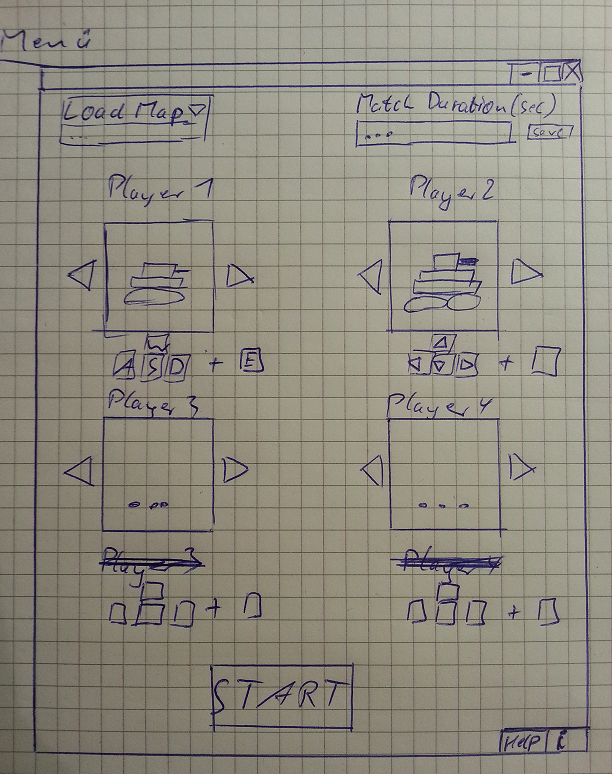
\includegraphics[width=10cm]{menu_entwurf.png}
 \caption{Spielfigur aus Vorschau aller verfügbaren Figuren auswählen. Information über jeweilige Spielfigur verfügbar. Tastenbelegung unter Vorschau angezeigt. Default: Keine Figur ausgewählt, Anzahl Spieler bestimmt durch Anzahl ausgewählter Figuren. Match Duration in Sekunden eingeben}
\end{figure}

\begin{figure}[H]
\textbf{Game Screen Entwurf:}\par\medskip
\centering
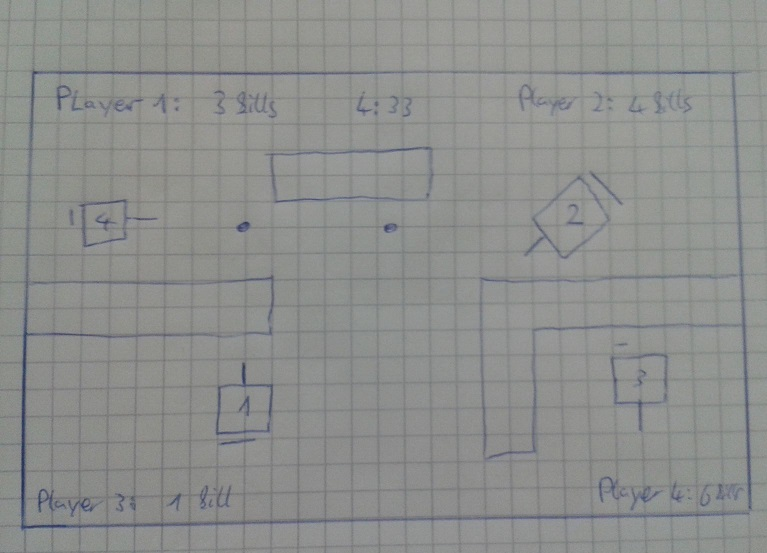
\includegraphics[width=15cm]{game_entwurf.jpg}
\caption{Anzeige der verbleibenden Spielzeit mittig am oberen Spielfeldrand; Anzeige der Abschüsse und Tode der Spieler in den Ecken; Hindernisse, die nicht durchfahren werden können; Spielfiguren feuern Projektile}	
\end{figure}


\section{Qualitätsziele}
\begin{itemize}
\item Spiel läuft flüssig und von der CPU Geschwindigkeit unabhängig
\item Einfache Bedienung durch den Benutzer
\item Figuren leicht steuerbar
\end{itemize}